\section{The IGE Rises With Age}\label{sec:ageprofile}

The IGE of sons' earnings rises by three quarters between the late twenties and the forties. In the PSID it is
0.276$^{***}$ at 25--29 and 0.492$^{***}$ at 40--44, and it stays near that level to 55 (0.498$^{***}$ at 50--55) (Table~\ref{tab:ige_sons}). The
same sons followed from 25 to 49 show the same rise, and so do two other cohorts in the NLSY79 and the NLSY97. Ranks of
family income rise only into the early thirties, so the 31--37 window of \citet{chetty2020race} lies on the plateau of the
rank profile and before the end of the log profile's rise. The rise is White: the IGE of Black sons is flat in age.

\subsection{The profile}

Pooled across races and weighted, the IGE of sons' own earnings is 0.276$^{***}$ (0.024) at 25--29, 0.403$^{***}$ at
30--34, 0.454$^{***}$ at 35--39, 0.492$^{***}$ at 40--44 and 0.484$^{***}$ at 45--49; that of their family income goes
from 0.301$^{***}$ (0.023) to 0.530$^{***}$ at 40--44. Equality across bands is rejected ($\chi^2(5) = 45.3$,
$p<0.001$), the trend is 0.078$^{***}$ (0.022) per ten years of age, and the mean IGE from 35 exceeds the mean below 35
by 0.142$^{***}$ ($p<0.001$).\footnote{Sons with parental income over at least three years of their ages 13--19, child-year
regressions within each band with single-age dummies, PSID weights, standard errors clustered by 1968 family. Code:
\texttt{26.IGEByAge.py} (\texttt{output/ige\_by\_age.md}, Sections 1a and 2).}

\begin{table}[!htbp]
\centering
\caption{Log IGE of sons' income by age at measurement (PSID)}
\label{tab:ige_sons}
\resizebox{\ifdim\width>\textwidth\textwidth\else\width\fi}{!}{%
\resizebox*{!}{\ifdim\totalheight>0.85\textheight 0.85\textheight\else\totalheight\fi}{%
\begin{tabular}{lcc}
\toprule
Age band / group & \begin{tabular}[b]{@{}c@{}}ln own earnings\\(child-years)\end{tabular} & \begin{tabular}[b]{@{}c@{}}ln family income\\(child-years)\end{tabular} \\
 & (1) & (2) \\
\midrule
\multicolumn{3}{l}{\textit{Age 25--29}} \\
Pooled (weighted) & $0.276^{***}$ & $0.301^{***}$ \\
 & (0.024) & (0.023) \\
Black & $0.262^{***}$ & $0.266^{***}$ \\
 & (0.036) & (0.034) \\
White & $0.221^{***}$ & $0.250^{***}$ \\
 & (0.028) & (0.026) \\
White $-$ Black & $-0.041$ & $-0.016$ \\
 & (0.045) & (0.043) \\
Children (Black / White) & 1,607 / 2,474 & 1,662 / 2,506 \\
\addlinespace
\multicolumn{3}{l}{\textit{Age 30--34}} \\
Pooled (weighted) & $0.403^{***}$ & $0.451^{***}$ \\
 & (0.027) & (0.027) \\
Black & $0.282^{***}$ & $0.283^{***}$ \\
 & (0.037) & (0.040) \\
White & $0.369^{***}$ & $0.419^{***}$ \\
 & (0.031) & (0.031) \\
White $-$ Black & $0.087^{*}$ & $0.137^{***}$ \\
 & (0.048) & (0.050) \\
Children (Black / White) & 1,415 / 2,253 & 1,477 / 2,295 \\
\addlinespace
\multicolumn{3}{l}{\textit{Age 35--39}} \\
Pooled (weighted) & $0.454^{***}$ & $0.501^{***}$ \\
 & (0.031) & (0.032) \\
Black & $0.259^{***}$ & $0.313^{***}$ \\
 & (0.044) & (0.048) \\
White & $0.431^{***}$ & $0.464^{***}$ \\
 & (0.037) & (0.035) \\
White $-$ Black & $0.173^{***}$ & $0.151^{**}$ \\
 & (0.058) & (0.060) \\
Children (Black / White) & 1,068 / 1,838 & 1,125 / 1,884 \\
\addlinespace
\multicolumn{3}{l}{\textit{Age 40--44}} \\
Pooled (weighted) & $0.492^{***}$ & $0.530^{***}$ \\
 & (0.037) & (0.034) \\
Black & $0.197^{***}$ & $0.246^{***}$ \\
 & (0.050) & (0.055) \\
White & $0.491^{***}$ & $0.489^{***}$ \\
 & (0.044) & (0.043) \\
White $-$ Black & $0.294^{***}$ & $0.244^{***}$ \\
 & (0.067) & (0.070) \\
Children (Black / White) & 751 / 1,411 & 808 / 1,472 \\
\bottomrule
\end{tabular}}}
\par\smallskip
\begin{minipage}{\textwidth}\footnotesize \textit{Continued on the next table; notes below its last part.}\end{minipage}
\end{table}
\begin{table}[!htbp]
\centering
\addtocounter{table}{-1}
\caption{Log IGE of sons' income by age at measurement (PSID) (continued)}
\resizebox{\ifdim\width>\textwidth\textwidth\else\width\fi}{!}{%
\resizebox*{!}{\ifdim\totalheight>0.85\textheight 0.85\textheight\else\totalheight\fi}{%
\begin{tabular}{lcc}
\toprule
Age band / group & \begin{tabular}[b]{@{}c@{}}ln own earnings\\(child-years)\end{tabular} & \begin{tabular}[b]{@{}c@{}}ln family income\\(child-years)\end{tabular} \\
 & (1) & (2) \\
\midrule
\multicolumn{3}{l}{\textit{Age 45--49}} \\
Pooled (weighted) & $0.484^{***}$ & $0.481^{***}$ \\
 & (0.051) & (0.049) \\
Black & $0.213^{***}$ & $0.215^{***}$ \\
 & (0.064) & (0.072) \\
White & $0.511^{***}$ & $0.473^{***}$ \\
 & (0.060) & (0.061) \\
White $-$ Black & $0.299^{***}$ & $0.258^{***}$ \\
 & (0.088) & (0.095) \\
Children (Black / White) & 496 / 1,001 & 557 / 1,051 \\
\addlinespace
\multicolumn{3}{l}{\textit{Age 50--55}} \\
Pooled (weighted) & $0.498^{***}$ & $0.534^{***}$ \\
 & (0.063) & (0.056) \\
Black & $0.269^{***}$ & $0.290^{***}$ \\
 & (0.074) & (0.089) \\
White & $0.487^{***}$ & $0.478^{***}$ \\
 & (0.073) & (0.070) \\
White $-$ Black & $0.218^{**}$ & $0.187^{*}$ \\
 & (0.103) & (0.114) \\
Children (Black / White) & 351 / 726 & 420 / 780 \\
\addlinespace
\multicolumn{3}{l}{\textit{Age 31--37 (window of Chetty et al.)}} \\
Pooled (weighted) & $0.424^{***}$ & $0.475^{***}$ \\
 & (0.027) & (0.028) \\
Black & $0.292^{***}$ & $0.303^{***}$ \\
 & (0.036) & (0.041) \\
White & $0.392^{***}$ & $0.437^{***}$ \\
 & (0.032) & (0.031) \\
White $-$ Black & $0.099^{**}$ & $0.134^{***}$ \\
 & (0.048) & (0.051) \\
Children (Black / White) & 1,399 / 2,205 & 1,460 / 2,246 \\
\bottomrule
\end{tabular}}}
\par\smallskip
\begin{minipage}{\textwidth}\footnotesize \textit{Notes:} Each cell is the coefficient on log parental family income (mean over the child's ages 13--19) from a separate regression of the outcome in the column header, within the age band of the panel. Child-year columns: child-years in the band, controls for a quartic in the parent's age and single-year age dummies; band-mean columns (daughters' table; for sons in \texttt{output/ige\_by\_age.md}): one observation per child, log of the band mean ($\geq 2$ years), quartic in the parent's age and the mean age. Black and White: unweighted; Pooled: all races, weighted by the core longitudinal weight. White $-$ Black is the difference of the two race-specific regressions, estimated jointly. Standard errors clustered by 1968 family in parentheses. Race is the race of the parental household head. $^{***}$ $p<0.01$, $^{**}$ $p<0.05$, $^{*}$ $p<0.1$. Source: \texttt{26.IGEByAge.py} (\texttt{output/ige\_by\_age.csv}); table built by \texttt{28.PaperBTables.py}.\end{minipage}
\end{table}


The rise is not a change in who is observed. In the panel of sons observed in every band of 25--49 the earnings IGE is
0.272$^{***}$ at 25--29, 0.386$^{***}$ at 30--34, 0.432$^{***}$ at 35--39, 0.473$^{***}$ at 40--44 and 0.478$^{***}$ at
45--49, a trend of 0.100$^{***}$ (0.027) per ten years. It is the intergenerational face of the life-cycle bias of
\citet{haider2006life}: following the same sons from 25--29 to 35--39, their family income grows faster with parental
income by 0.210$^{***}$ (0.031), whereas between 30--34 and 40--44 the growth gradient is 0.021 (0.036), so the rise is
concentrated before the mid-thirties.\footnote{Appendix Table~\ref{tab:growth}; \texttt{output/ige\_by\_age.md},
Sections 1b and 5.1.} Nor is it calendar time. The rise from 25--29 to 45--49 is 0.216$^{***}$ among sons born 1951--64,
0.147$^{*}$ among those born 1965--79 and 0.165$^{*}$ to 40--44 among those born 1980--89, cohorts observed at the same ages
in different decades; it is 0.192$^{***}$ with income-year fixed effects in every band and 0.240$^{***}$ in a fixed
window of income years 1990--2010, in which the bands hold different cohorts (panel A of Table~\ref{tab:age_period}).

\begin{table}[!htbp]
\centering
\caption{Age or period? The pooled rise of the IGE and the son's AFQT in two cohorts}
\label{tab:age_period}
\resizebox{\ifdim\width>\textwidth\textwidth\else\width\fi}{!}{%
\resizebox*{!}{\ifdim\totalheight>0.85\textheight 0.85\textheight\else\totalheight\fi}{%
\begin{tabular}{lccc}
\toprule
 & \begin{tabular}[b]{@{}c@{}}25--29\end{tabular} & \begin{tabular}[b]{@{}c@{}}45--49\end{tabular} & \begin{tabular}[b]{@{}c@{}}Rise\end{tabular} \\
 & (1) & (2) & (3) \\
\midrule
\multicolumn{4}{l}{\textit{A. PSID sons, ln earnings, IGE by band}} \\
Baseline & $0.283^{***}$ & $0.492^{***}$ & $0.209^{***}$ \\
 & (0.025) & (0.052) & (0.050) \\
Born 1951--64 & $0.296^{***}$ & $0.512^{***}$ & $0.216^{***}$ \\
 & (0.035) & (0.061) & (0.060) \\
Born 1965--79 & $0.299^{***}$ & $0.446^{***}$ & $0.147^{*}$ \\
 & (0.051) & (0.082) & (0.076) \\
Born 1980--89 (to 40--44) & $0.290^{***}$ & $0.455^{***}$ & $0.165^{*}$ \\
 & (0.045) & (0.085) & (0.086) \\
Income-year fixed effects & $0.298^{***}$ & $0.490^{***}$ & $0.192^{***}$ \\
 & (0.024) & (0.053) & (0.050) \\
IGE $\times$ cohort, at the 1965 cohort & $0.303^{***}$ & $0.491^{***}$ & $0.187^{***}$ \\
 & (0.027) & (0.053) & (0.050) \\
Period-varying IGE, at 1995 & $0.294^{***}$ & $0.593^{***}$ & $0.300^{***}$ \\
 & (0.025) & (0.084) & (0.084) \\
Income years 1990--2010 only & $0.286^{***}$ & $0.525^{***}$ & $0.240^{***}$ \\
 & (0.038) & (0.058) & (0.066) \\
\addlinespace
\multicolumn{4}{l}{\textit{B. The son's AFQT in the IGE of ln earnings (columns 1--2: 25--29 and 40--44)}} \\
NLSY97 (born 1980--84): IGE & $0.175^{***}$ & $0.258^{***}$ &  \\
 & (0.021) & (0.027) &  \\
NLSY97: son's AFQT contribution & $0.033^{***}$ & $0.054^{***}$ &  \\
 & (0.006) & (0.010) &  \\
NLSY79 (born 1957--64): son's AFQT contribution & $0.077^{***}$ & $0.131^{***}$ &  \\
 & (0.010) & (0.014) &  \\
\bottomrule
\end{tabular}}}
\par\smallskip
\begin{minipage}{\textwidth}\footnotesize \textit{Notes:} Panel A: Black and White sons pooled with PSID weights, ages 25--49; single-age dummies and the parent's age quartic; rise = 45--49 minus 25--29 (40--44 for the 1980--89 cohort); standard errors clustered by 1968 family. Panel B: exact Gelbach split with the son's AFQT as its own group (NLSY97: ASVAB math-verbal percentile, standardised within birth year; parental income = the 1996 parent report; NLSY79: AFQT-3, 1979--81 parental income); 200 cluster-bootstrap draws of households. Source: \texttt{95.PooledRiseChecks.py}, \texttt{94.NLSY97AFQT.py}, \texttt{87.NLSY79YouthAFQT.py}; table built by \texttt{100.PaperBFableTables.py}. $^{***}$ $p<0.01$, $^{**}$ $p<0.05$, $^{*}$ $p<0.1$.\end{minipage}
\end{table}
 It replicates in the NLSY79, where the earnings IGE of sons born 1957--64 rises from 0.340$^{***}$ at
25--29 to 0.506$^{***}$ at 50--54 (an opening of 0.166$^{***}$, $p<0.001$), and in the NLSY97 (a trend of 0.063$^{***}$ over
25--44). Daughters' family income shows the same rise (Appendix Tables~\ref{tab:ige_daughters} and \ref{tab:nlsyage}).

\subsection{Ranks}

Ranks rise less and earlier. The rank--rank slope of sons' family income is 0.328$^{***}$ (0.020) at 25--29 and
0.427$^{***}$ at 30--34, and then flat: 0.436$^{***}$ at 35--39, 0.423$^{***}$ at 40--44 and 0.380$^{***}$ at 45--49
(Appendix Table~\ref{tab:rankage}). The PSID slope in the 31--37 window, 0.442$^{***}$, lies on the plateau. Logs and
ranks differ because the log IGE also registers the dispersion of sons' log income relative to their parents', which
grows with age and which ranks normalise away.\footnote{Within the same children and weights, the widening of the
log profile is mostly the ratio of the standard deviations of children's and parents' log income;
\texttt{output/ige\_by\_age.md}, Section 5.4.} An IGE measured at 31--37 therefore captures the whole rise in ranks and
stops before the log IGE reaches its level of the forties.

\subsection{By race}

The rise is concentrated among White sons (Figure~\ref{fig:headline}). The earnings IGE of White sons climbs from
0.221$^{***}$ at 25--29 to 0.431$^{***}$ at 35--39 and 0.511$^{***}$ at 45--49; that of Black sons is 0.262$^{***}$ at
25--29 and between 0.20 and 0.28 at every later age. The White--Black gap is $-0.041$ (0.045) at 25--29 and
0.299$^{***}$ at 45--49, and its opening, the mean gap from 35 minus the mean gap below 35, is 0.232$^{***}$ (0.052) on
bands 25--49.\footnote{Table~\ref{tab:ige_sons} and Appendix Table~\ref{tab:agetests}. Code: \texttt{26.IGEByAge.py};
figure: \texttt{31.PaperBFigure.py}.} \citet{chetty2020race} measure rank--rank slopes of 0.28 for Black and 0.32 for
White children at 31--37 and expected ranks at the 25th parental percentile of 32.6 and 45.2; in the PSID these are
points on rank profiles that are flat in age for both races. The racial opening in logs is robust to cohorts, period
effects, attrition weights, an experience clock and a dollar-weighted elasticity, and with one year of parental income it
is about 0.09 log points in four public data sets, 0.19 corrected for the unreliability of that year (Appendix~\ref{app:race}).
Sections~\ref{sec:passedon}--\ref{sec:stability} ask which components of what parents pass on carry the rise, and for
whom.

\begin{figure}[!htbp]
\centering
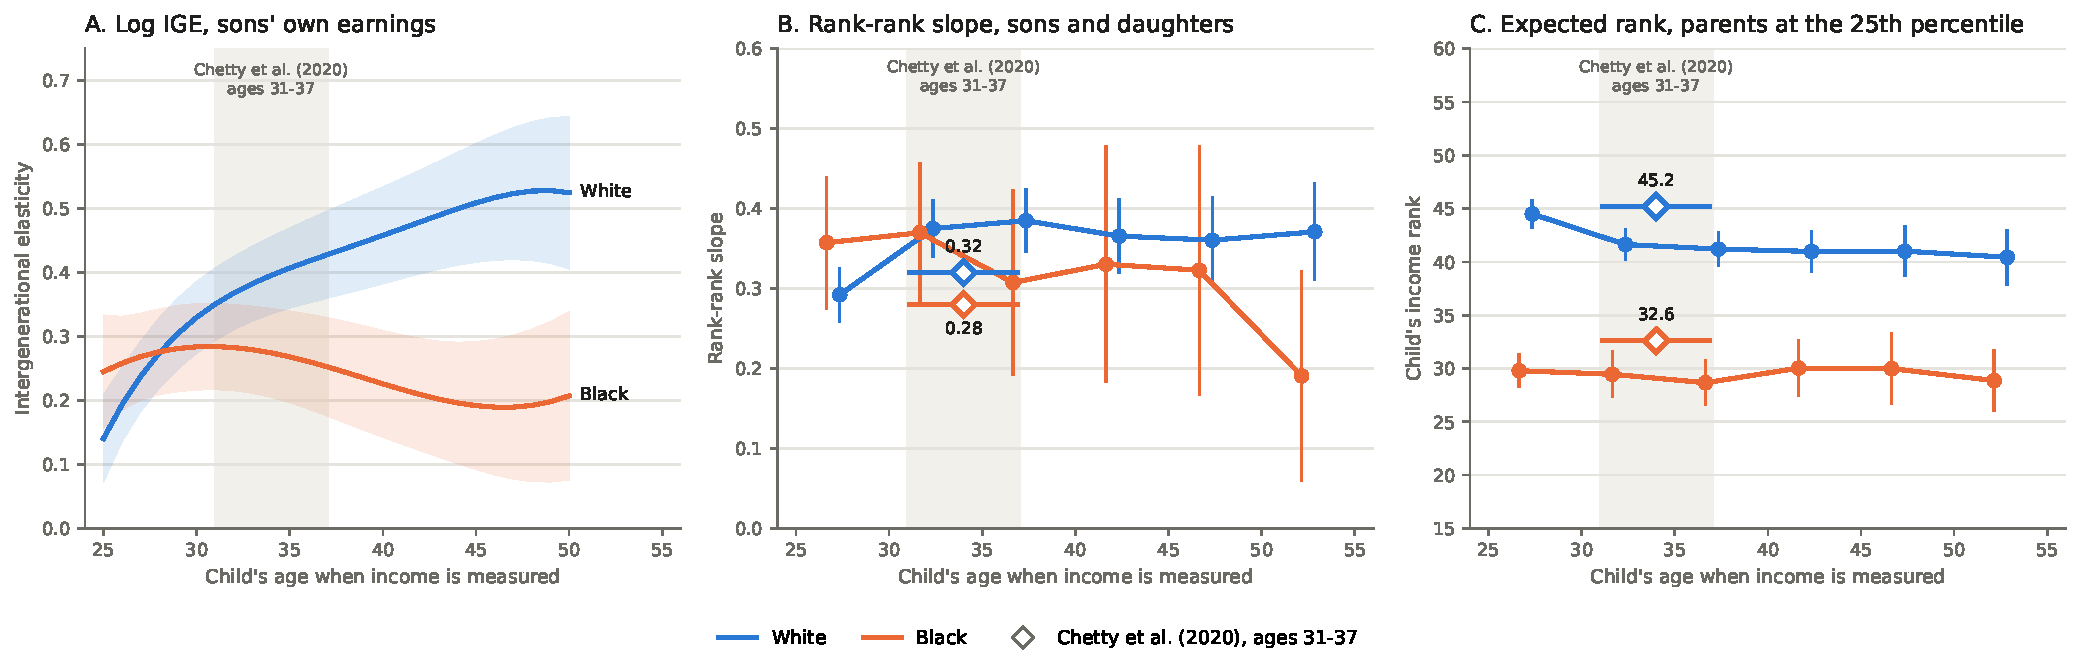
\includegraphics[width=\textwidth]{paperB_age_profile.pdf}
\caption{The age profile of intergenerational persistence, with \citet{chetty2020race} placed on it (PSID)}
\label{fig:headline}
\begin{minipage}{\textwidth}\footnotesize \textit{Notes:} Panel A: log IGE of sons' own earnings at each age, Black
and White, from one Lee--Solon regression with parental income interacted with a quartic in the son's age (child-years
at 25--55; ages above 50 not plotted), 95\% confidence bands. Panel B: rank--rank slope of household income by age band,
sons and daughters, weighted. Panel C: expected household income rank of children whose parents are at the 25th
percentile, by age band. Diamonds: \citet{chetty2020race} at 31--37. Shaded: the 31--37 window. Code:
\texttt{26.IGEByAge.py} (estimates) and \texttt{31.PaperBFigure.py} (figure).\end{minipage}
\end{figure}
